\chapter*{Búsqueda binaria}
\markboth{Búsqueda binaria}{Búsqueda binaria}
\addcontentsline{toc}{chapter}{Búsqueda binaria}

Esta técnica es una de las más poderosas e importantes en la informática. Es una forma muy eficiente de hacer búsquedas que nos permite resolver problemas antes imposibles.

Utilizada en muchas aplicaciones, nos permite resolver problemas donde una búsqueda completa tardaría miles de millones de años en menos de un segundo. Y esta impresionante herramienta ahora será tuya.

La búsqueda binaria difiere de la completa al evitar revisar absolutamente todas las opciones del espacio de búsqueda. Si no, lo que hace es que en cada paso logra descartar la mitad del espacio de búsqueda al darse cuenta que la respuesta no está allí.

Porque en cada paso va descartando la mitad de las opciones, llega a una única opción (la respuesta si esta existe) en muy poco tiempo. Mientras que la búsqueda completa va eliminando opciones de una en una.

Comparemos un ejemplo de la búsqueda completa vs la binaria, si tuviéramos \(128\) candidatos. 

\begin{center}
	\begin{tabular}{|c|c|c|}
		\hline
		\multirow{2}{*}{\shortstack{Número\\ de pasos}} & \multicolumn{2}{c|}{Candidatos restantes} \\
		\cline{2-3}
		 & Completa & Binaria \\
		\hline
		0 & 128 & 128  \\		
		\hline
		1 & 127 & 64  \\		
		\hline
		2 & 126 & 32  \\
		\hline
		3 & 125 & 16  \\
		\hline
		4 & 124 & 8  \\
		\hline
		5 & 123 & 4  \\
		\hline
		6 & 122 & 2  \\
		\hline
		7 & 121 & 1  \\
		\hline
		8 & 120 &   \\	
		\multicolumn{3}{c}{
	\begin{LARGE}
	
		\(\cdots\)
		
	\end{LARGE} 
	}\\
		125 & 3 &  \\		
		\hline
		126 & 2 &  \\		
		\hline
		127 & 1 &  \\
		\hline
	\end{tabular}
\end{center}

Como vemos, búsqueda binaria pudo reducir los candidatos a solo uno con siete pasos, mientras que la búsqueda completa requirió de 127.

El motivo por el cuál la búsqueda binaria es tan efectiva, es que realiza \(\lceil log_2(candidatos) \rceil\) pasos \footnote{\(\lceil log_2(A) \rceil \) significa: techo del logaritmo base dos de A.\\ Recordemos que \(log_2(A)=x\) significa que \(2^x=A\).\\ Y el techo nos dice que tomemos el menor entero que sea mayor igual que el valor de adentro, por ejemplo:. \(\lceil 3.12 \rceil =4\)}. Esto es porque \(\lceil log_2 \rceil \) nos permite calcular cuantas veces podemos dividir un número entre dos hasta que sea 1.

Veamos un ejemplo que se puede resolver con búsqueda binaria.
\pagebreak
\section*{Ejemplo 3.1}
\addcontentsline{toc}{section}{Ejemplo 3.1}

Javier es un granjero y esta cansado de que sus animales siempre huyan de su granja, por lo que ha decidido poner una reja al rededor de todo el terreno.

Sin embargo, Javier no sabe cuantos metros de reja va a necesitar y te ha contratado para que tu le digas esto. 

Lo que él si sabe es que el tiene forma cuadrada con lados de longitud entera, además recuerda que este mide \(A\) metros cuadrados de área.

Ayuda a Javier para que sepa cuanta reja necesita.

\subsection*{Entrada}
Un entero \(A\), el tamaño del terreno en metros cuadrados.
\subsection*{Salida}
Un entero indicando cuantos metros de reja necesita para rodear todo el terreno. 

\subsection*{Ejemplos}
\begin{casebox2}
	\scase{36}{24}
	\scase{100}{40}
	\scase{1}{4}
\end{casebox2}

\subsection*{Límites}
\begin{plimits}
	\item \(1\leq A \leq 10^{18}\)
\end{plimits}
\subsection*{Subtareas}
\begin{plimits}
	\item (35 pts) \(1\leq A \leq 10^9\)
	\item (65 pts) Sin restricciones adicionales
\end{plimits}

\subsection*{Solución}
Como siempre, antes de leer la solución te invitamos a que intentes el problema.


En este problema nos piden de que dado el área de un cuadrado, imprimamos el perímetro. Por esto, recordemos las formulas del cuadrado.
\[Per\acute{i}metro=4\times Lado \]
\[\acute{A}rea=Lado\times Lado \]

Entonces, si encontramos el lado que nos de el área de entrada, podremos encontrar el perímetro.

Para este problema vamos a ver dos estrategias para resolverlo, la de búsqueda lineal y la binaria.

Comencemos con la que ya deberíamos estar familiarizada, usemos búsqueda lineal.

\subsubsection*{Búsqueda lineal}
Entonces, buscaremos el entero \(L\) de entre todos los posibles, que cumpla que \(A=4\times L\). Para esto, podremos ir probando del \(1\) en adelante hasta encontrar el que cumpla.

\begin{lstlisting}
	long long L=1;
	while (L*L != A) {
		L++;
	}
\end{lstlisting}

Esto itera por todos los enteros del \(1\) a la respuesta que es \(\sqrt{A}\). Por lo tanto, su complejidad es \(O(\sqrt{A})\). Lo cual corre para la subtarea de 35 puntos, pero no para el límite completo de \(10^{18}\).

\subsubsection*{Búsqueda binaria}
Ahora resolvamos el problema utilizando búsqueda binaria.

Definamos nuestro espacio de búsqueda, ¿cuáles valores puede ser \(L\)? y si lo pensamos puede ser desde \(1\) hasta \(10^9\). Porque \(10^9\times 10^9=10^{18}\) y de los límites sabemos que \(1\leq A\leq 10^{18}\).

Entonces queremos encontrar la respuesta que esta entre \(1\) y \(10^9\), hagamos una función que logre esto llamada buscar que reciba el rango de donde esta la respuesta.

\begin{lstlisting}
	//Encuentra L tal que L*L=A, sabiendo que a<=L<=b.
	long long buscar(long long a, long long b, long long A);
\end{lstlisting}

Ahora tenemos \(10^9\) candidatos donde encontrar la respuesta y queremos reducirlo a la mitad. 

Para esto podemos ver que sucede con \(5\times10^8\). 

Si resulta que \((5\times10^8)\times(5\times10^8) <A\), entonces sabemos que cualquier valor menor igual que \(5 \times 10^8\) no funcionará porque es demasiado pequeño. Por lo tanto la respuesta debe estar entre \(5\times 10^8 +1\) y \(10^9\) y los candidatos se redujeron a la mitad.

Pero si en vez sucede que \((5\times10^8)\times(5\times10^8) >=A\), entonces sabremos que cualquier valor más grande que \(5\times 10^8\) nos dará valores más grandes que \(A\) y por lo tanto la respuesta no estará allí. Ahora nuestros candidatos son los números entre \(1\) y \(5\times 10^8\), reduciendo los valores que podrían ser la respuesta a la mitad.

Y de hecho, si en general, la respuesta esta entre \(a\) y \(b\), nos convendrá preguntar por el punto medio \((a+b)/2\), que nos reducirá el espacio a la mitad.

Una vez que redujimos el rango de la búsqueda, tendremos que encontrar la respuesta en ese nuevo rango, y para esto podemos hacer recursión.

De forma que ahora tenemos:
\begin{lstlisting}
	long long buscar(long long a, long long b, long long A) {
		long long m =(a+b)/2;
		if (m*m < A) {
			return buscar(m+1, b, A);
		} else {
			return buscar(a, m, A);
		}
	} 
\end{lstlisting}

Ahora, lo que le falta a esa recursión es una condición de paro, saber cuando ya termino y encontramos la respuesta.

Podremos ver que habremos encontrado la respuesta cuando ya estemos seguros de cual es esta. Y esto sucede cuando nuestro rango solo incluye un valor, es decir, cuando \(a==b\) se cumpla.

\begin{lstlisting}
	long long buscar(long lonng a, long long b, long long A) {
		if (a==b)
			return a;
		long long m=(a+b)/2;
		if (m*m<A) {
			return buscar(m+1, b, A);
		} else {
			return buscar(a, m, A);
		}
	}
\end{lstlisting}

Y con esto, tenemos que \verb|L=buscar(1, 1000000000, A)|.

Ahora, la complejidad de esto es \(O(log(\sqrt{A}))\), lo cual corre perfectamente para \(10^{18}\).

\paragraph{Nota:} En este problemas también se pudo haber usado \verb|L=sqrt(A)| con la librería \verb|<math.h>| que calcula el valor rápidamente, pero se uso búsqueda binaria para ejemplificar.


\section*{Ejemplo 3.2}
\addcontentsline{toc}{section}{Ejemplo 3.2}
Se te da un arreglo \(A\) de \(N\) enteros diferentes. El arreglo estará en orden creciente, es decir, \(A[i] < A[i+1]\).

Deberás responder \(T\) preguntas:

Cada pregunta consistirá de un entero \(q_i\) y tu deberás imprimir el índice del valor \(q_i\) o \(-1\) si este valor no existe.
\subsection*{Entrada}
El enteros \(N\).

En la siguiente línea: \(N\) enteros separados, los valores del arreglo \(A\).

En la siguiente línea recibirás el entero \(T\).

En las siguientes \(T\) líneas recibirás los valores de cada pregunta.

\subsection*{Salida}
Imprime la respuesta cada pregunta en una línea en el mismo orden que el de lectura.

\subsection*{Ejemplo}
\begin{casebox2}
	\scase{
		7\\
		2 5 6 7 8 9 10\\
		5\\
		2\\
		6\\
		4\\
		10\\
		5\\
	}
	{
		0\\
		2\\
		-1\\
		6\\
		1		
	}
\end{casebox2}
\subsection*{Límites}
\begin{plimits}
	\item \(1\leq N,T \leq 10^5 \)
	\item \(1\leq A[i], q_i \leq 10^9 \)
\end{plimits}

Enlace: TODO

\subsection*{Solución}
Esta ocasión nos piden encontrar el indice de un valor en un arreglo ordenado. Ya hemos visto como hacerlo con búsqueda lineal:

\begin{lstlisting}
	int indice(int q) {
		for (int i =0; i < N;i++) 
			if (A[i]==q)
				return i;
		return -1;
	}
\end{lstlisting}

Sin embargo, esto no corre en tiempo ya que la complejidad es \(O(N)\) por pregunta, siendo en total \(O(TN)\) y como \(TN=10^{10}\), obtendremos TLE.

Pero veamos que podemos usar búsqueda binaria. ya que al preguntar por una posición de en medio y discernir si tenemos que buscar adelante o atrás.

\begin{lstlisting}
	int binaria(int a, int b, int q) {
		if (a>b)
			return -1;
		int m =(a+b)/2;
		if (A[m]==q)
			return m;
		if (A[m]<q) {
			return binaria(m+1, b, q);
		} else {
			return binaria(a, m-1, q);
		}		
	}
	int indice(int q) {
		return binaria(0, N-1, q);
	}
\end{lstlisting}

La nueva complejidad ahora es \(O(logN)\) por pregunta, en total\\ \(O(TlogN)\)

\section*{Dificultades}
\addcontentsline{toc}{section}{Dificultades}
Ya vimos que la búsqueda binaria tiene una ventaja enorme sobre la búsqueda lineal ya que resuelve el problema en un tiempo mucho menor.

Pero tristemente, no siempre es posible aplicar la búsqueda binaria. Hay veces en que las que no se puede descartar fácilmente la mitad de los candidatos.

Un caso donde puede suceder sería en el ejemplo anterior si el arreglo no estuviese ordenado. En ese caso no podríamos hacer el truco de solo revisar adelante si \(A[m]<q\) ya que no nos da suficiente información esa pregunta para eliminar todos los valores de \(0\) a \(m\).

Por supuesto, el problema anterior tiene corrección para que la búsqueda binaria siga funcionando y muchas veces esto es parte del problema, ¿cómo hago la binaria aquí? Pero hay otras veces que es imposible, o al menos, más allá de los conocimientos actuales.

En esos casos, no quedará de otra más que hacer búsqueda completa o usar una técnica diferente a búsqueda.

Otro ejemplo donde la búsqueda binaria no se puede utilizar es en encontrar el primer divisor que no sea 1 de un entero.
\newpage

\practiceproblemsection{3}

\problemtitle Fernando es el operador de montacargas en un almacén cuando le pidieron que sacara \(K\) piezas del inventario.

Sin embargo, las piezas están organizadas en una pila de \(N\) cajas. La caja \(i\) contiene \(C_i\) piezas.

Como funciona el montacargas, Fer puede agarrar las primeras \(R\) cajas de la pila y traerlas consigo.

Es decir, si \(C=[1,2,3,4]\) y \(R=2\), el montacargas se llevará las cajas \([1,2]\).

Como el montacargas gasta gasolina según cuantas cajas cargue y esta es muy cara, ayuda a Fer a determinar la mínima \(R\) para \(Q\) valores de \(K\).

\subsubsection*{Entrada}
Un entero \(N\) representando la cantidad de cajas.

En la siguiente línea habrá \(N\) enteros, los valores de \(C_1, C_2, \ldots, C_N\).

En la tercera línea estará el entero \(Q\), para cuantos valores debes descubrir \(R\).

En las siguientes \(Q\) líneas habrá un entero \(K\) que representa la cantidad de piezas deseada, suponiendo que siempre tenemos las mismas \(N\) cajas.

\subsubsection*{Salida}

Por cada una de las \(Q\) preguntas: imprime una línea con la mínima \(R\) para obtener \(K\) piezas, si no se puede imprime \(-1\).

\subsubsection*{Ejemplo}

\begin{casebox3}
	\ecase{
		3\\
		1 4 1\\
		3\\
		1\\
		3\\
		10
	}{
		1\\
		2\\
		-1
	}{
		Agarrando la caja No. 1 obtenemos 1 pieza\\ 
		\\
		Tomando la caja No. 1 y No. 2, tenemos 5\\ piezas, las cuales son mas que 3.\\
		\\
		No hay suficientes piezas para 10.
	}
	\ecase{
		5\\
		3 1 1 3 1\\
		1\\
		4
	}{
		2
	}{}
\end{casebox3}
\subsubsection*{Límites}
\begin{plimits}
	\item Para 50\%
	\begin{plimits}
		\item \(0< N \leq 10^2\)
		\item \(0< Q \leq 10^3\)
	\end{plimits}
	\item Para 100\%
	\begin{plimits}
		\item \(0< N \leq 10^5\)
		\item \(0< Q \leq 10^5\)
		\item \(0< C_i \leq 1000\)
		\item \(0\leq K \leq 10^9\)
	\end{plimits}
\end{plimits}

Enlace: \omegalink{Transporte-de-Cajas}



\problembreak

\problemtitle Sho colecciona juegos de dominó y quiere jugar.

Pero los dominós de Sho son un poco especiales, ya que son k-dominós. El dominó tradicional es del tipo 6-dominó, porque tiene números del \(0\) al \(6\), con un total de 28 fichas.

Entonces, un k-dominó tendrá números del \(0\) al \(k\). Con una ficha por cada par posible de números, incluyendo las mulas (mula es el mismo número emparejado consigo mismo).

Las fichas del 6-dominó son:

\begin{center}
		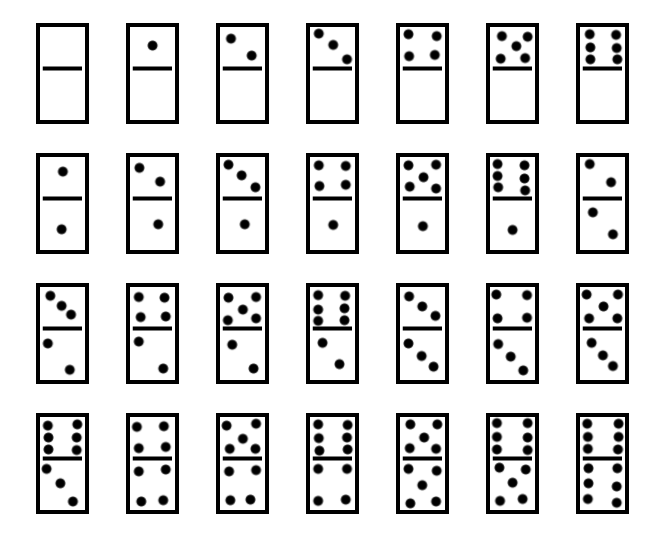
\includegraphics[scale=0.4]{domino6}
\end{center}

Y las del 2-domino son las siguientes seis:
\begin{center}
	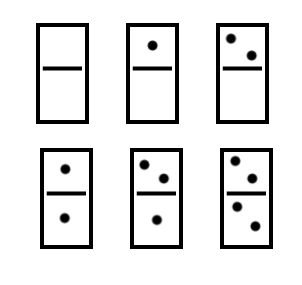
\includegraphics[scale=0.4]{domino2}
\end{center}

Sho quiere jugar con al menos \(N\) fichas, pero como después de jugar tiene que guardar, quiere usar el dominó con menor cantidad de fichas que tenga por lo menos \(N\) fichas. 

Dado \(N\), encuentra el valor de \(k\) para el k-dominó que le sirve a Sho.

\subsubsection*{Ejemplo}
\begin{casebox2}
	\scase{30}{6}
	\scase{6}{2}
	\scase{1000}{44}
\end{casebox2}

\subsubsection*{Límites}
\begin{plimits}
	\item \(1\leq N \leq 10^{18}\)
\end{plimits}

Enlace: TODO

\problembreak

\problemtitle Adivina el número que esta pensando OmegaUp.

Deberás implementar una función \verb|void adivina(long long a, long long b)| que descubra el número \(s\) que OmegaUp esta pensando. Se cumplirá que \(a\leq s\leq b\).

Para adivinar el número podrás llamar a la función \verb|long long pista(long long x)|.

Esta función regresará:
\begin{plimits}
	\item \verb|-1| si el número que piensa OmegaUp es menor que \(x\).
	\item \verb|0| si el número que piensa OmegaUp es \(x\).
	\item \verb|1| si el número que piensa OmegaUp es mayor que \(x\).
\end{plimits} 

La ultima llamada a pista debe ser con el número que OmegaUp esta pensando.

\subsubsection*{Límites}
\begin{plimits}
	\item \(-2^{61}\leq a,b \leq 2^{61}\)	
\end{plimits}
\subsubsection*{Evaluación}
Tu puntuación será en base a la cantidad de llamadas que hagas a la función \verb|long long pista(long long x)| de la siguiente manera:
\begin{plimits}
	\item 100\% si haces a lo más \(log(b-a+1)\)llamadas
	\item 50\% si haces a lo más \(2log(b-a+1)\)llamadas
	\item 0\% si haces más de \(2log(b-a+1)\)llamadas
\end{plimits}

Enlace: \omegalink{COMI-Adivina-el-numero}

NOTA: Este es un problema interactivo, si no conoces como trabajar con estos, ve la página: \pageref{interactivos}

\problembreak

\problemtitle A.R.C. Markland-N es un edificio alto con \(n\) pisos enumerados del \(1\) al \(n\). Entre cada dos pisos adyacentes existe una escalera que los conecta.

Es hora del almuerzo para nuestro sensei, Colin "ConneR" Neumann Jr, y él está planeando la ubicación donde disfrutar su comida.

La oficina de ConneR esta en el piso \(s\) del edificio. En cada piso (incluyendo \(s\)) hay un restaurante ofreciendo comida. Sin embargo, debido a renovaciones que están en proceso, \(k\) restaurantes se encuentran cerrados y por lo tanto, ConneR no puede disfrutar su almuerzo en ellos.

ConneR quiere llegar a un restaurante tan rápido como sea posible. ¿Cuál es el mínimo número de escaleras que debe usar para llegar al restaurante más cercano abierto?

\subsubsection*{Entrada}
En la primera línea habrá un entero \(t\) -- El número de casos pruebas. Luego vendrán las descripciones de cada uno de los \(t\) casos de prueba.

La primera línea de un caso de prueba tiene tres enteros \(n\), \(s\) y \(k\) -- Respectivamente, el número de pisos, el piso donde está ConneR y el número de restaurantes cerrados.

La segunda línea del caso de prueba tendrá \(k\) enteros distintos \(a_1, a_2 \ldots a_k\) -- Los números de piso con su restaurante cerrado.
\subsection*{Salida}

Por cada caso de prueba imprime una línea con la respuesta -- el mínimo número de escaleras que ConneR debe usar para llegar a un restaurante abierto.

\subsubsection*{Ejemplo}

\begin{casebox2}
	\scase{
		5\\
		5 2 3\\
		1 2 3\\
		4 3 3\\
		4 1 2\\
		10 2 6\\
		1 2 3 4 5 7\\
		2 1 1\\
		2\\
		100 76 8\\
		76 75 36 67 41 74 10 77		
	} {
		2\\
		0\\
		4\\
		0\\
		2
	}
\end{casebox2}
\subsubsection*{Límites}
\begin{plimits}
	\item\( 1 \leq t \leq 1000\)
	\item \(2\leq n \leq 10^9\)
	\item \(1\leq s \leq n\)
	\item \(1\leq k \leq min(n-1, 1000)\)
	\item Se garantiza que la suma de los valores de \(k\) no excederá \(1000\).
\end{plimits}

\codeforces

\codeforceslink{1293}{A}


\newpage
%------------------------------------------------------
\section*{Función de validación}
\addcontentsline{toc}{section}{Función de validación}
Igual que en búsqueda lineal podíamos agregar funciones más complicadas a la hora de buscar la respuesta, lo mismo sucede en búsqueda binaria. A veces requeriremos de más código que una simple comparación para saber en cual mitad esta la respuesta.

Veamos unos ejemplos.


\section*{Ejemplo 3.3}
\addcontentsline{toc}{section}{Ejemplo 3.4}
Karel ha comprado una bicicleta eléctrica con la que planea completar un recorrido. El recorrido se puede ver como \(N\) colinas en línea recta tal que la \(i\)-ésima colina tiene altura \(h_i\). Karel comienza en la colina hasta la izquierda y quiere terminar en la ultima colina de hasta la derecha.

Cuando Karel sube un metro gasta \(1\) unidad de energía, mientras que bajar un metro recupera \(1\) unidad de altura. Si Karel en algún momento necesita subir, pero su batería tiene 0 de energía, Karel se quedará atorado y no terminará el recorrido.

Por suerte al inicio hay una estación de recarga donde Karel puede recargar su bicicleta. Como nota, la batería tiene capacidad \(R\) y jamás podrá almacena más energía que \(R\).

Actualmente Karel tiene \(0\) de energía, Determina cuál es la menor cantidad de energía que es necesaria recargar al inicio para completar el recorrido. O determina si es imposible hacer el recorrido con la bicicleta de Karel.

\subsubsection*{Entrada}
La primera línea tiene dos enteros, el valor de \(N\) y \(R\).

En la siguiente línea vienen \(N\), enteros separados por espacios, siendo la altura de las colinas de izquierda a derecha. Recuerda que Karel comienza en la primera colina y quiera terminar en la última.
\subsubsection*{Salida}
Un entero, representando la menor cantidad de energía necesaria para completar el recorrido. Si Karel no puede completar el recorrido, imprime \(-1\).

\subsubsection*{Casos ejemplo}
\begin{casebox3}	
	\ecase{
		6 8\\
		4 6 3 5 7 
	}
	{3}
	{
		Karel inicia con 3 de energía, moverse de   \\
		la primera a la segunda colina le toma 2,  \\
		ahora tiene 1.\\
		Luego avanza y se recarga 3,\\
		ahora tiene 4.\\
		Después continua y se consume 2, ahora tiene 2. \\
		Vuelve a avanzar quedándose con 0 de energía. \\		
		Pero luego avanza y se recarga a 5. \\
		Finalmente avanza para termina con 5. \\
	}
	\ecase{
		5 6\\
		1 10 1 2 0
	}
	{-1}
	{}
	\hline
\end{casebox3}	

\subsubsection*{Límites}
\begin{plimits}
	\item \(2\leq N, R \leq 10^5\)
	\item \(0\leq h_i\leq 10^9\)
\end{plimits}

Fuente: OMIS online 2022.

Enlace: [TODO]

\section*{Solución}
Este problema 1.6 de búsqueda lineal con validación en la página \pageref{bicicleta}, si no sabes resolverlo con búsqueda lineal para los límites de allí, primero descubre esa solución.

Esta vez, los límites son más estrictos, de forma que la solución estándar con búsqueda lineal no funciona, pero veamos cual es porque nos será útil.
\\

La respuesta siempre estará entre \(0\)  y\(R\). La búsqueda lineal funciona de la siguiente manera.
\begin{lstlisting}
	int respuesta=-1;
	for (int e=0; e<=R; e++) {
		if (funciona(e)) {
			respuesta=e;
			break;
		}
	}
\end{lstlisting}

Y la función \verb|bool funciona(int e)| te regresa verdadero si Karel puede completar el recorrido comenzando con \(e\) de energía.

Esta función simplemente simula el recorrido para ver si Karel se atora en algún momento. Se ve de la siguiente forma:

\begin{lstlisting}
	bool funciona(int e) {
		for (int i = 1; i <N; i++){
			e-=A[i]-A[i-1];
			if (e > R) 
				e=R; //Limita la energia
			if (e < 0)
				return false;			
		}
		return true;
	}
\end{lstlisting}

La función \verb|funciona()| tiene una complejidad de \(O(N)\) y como es llamada en \(R\) valores, la complejidad total es \(O(RN)\).

Pero ahora veamos dos hechos importantes:
\begin{itemize}
	\item Si funciona(m) cumple, también lo hará cualquier valor mayor que \(m\).
	\item Si funciona(m) falla, también lo hará cualquier valor menor que \(m\).
\end{itemize}

Es decir, el rango de búsqueda se ve de la siguiente forma:

\begin{center}
	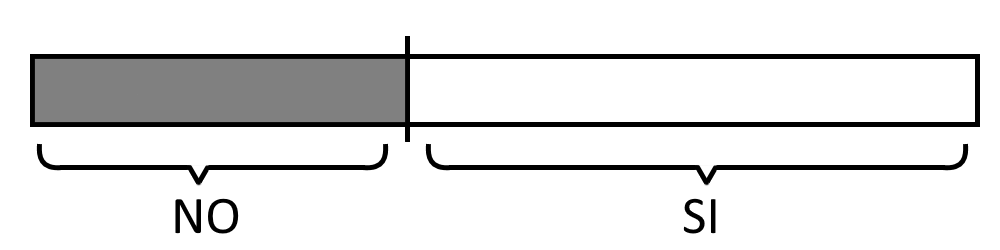
\includegraphics[scale=0.3]{binprop}
\end{center}

Esto hace que podamos hacer búsqueda binaria para encontrar el primer SI.

El código se verá como:

\begin{lstlisting}
	int a=0,b=R;
	while(a!=b) {
		int m=(a+b)/2;
		if (funciona(m)) {
			b=m;
		} else {
			a=m+1;
		}
	}
	int respuesta=-1;
	if (funciona(a))
		respuesta=a;
\end{lstlisting}

Ahora, recordemos que la complejidad de la búsqueda binaria es \(O(logR)\), pero en cada paso de la búsqueda estamos llamando a \verb|funciona()| que tiene complejidad \(O(N)\), por lo tanto, la complejidad total es \(O(NlogR)\).

\section*{Problemas de práctica}
\addcontentsline{toc}{section}{Problemas de práctica}

\problemtitle El COMI ha preparado un paseo por barco para los olímpicos del OMI por el río \textit{algorrio}. 

El concurso está organizado por \(M\) delegaciones enumeradas del \(1\) al \(M\), cada una con \(a_i\) olímpicos.

Para este paseo se planean contratar \(K\) barcos en el que se subirán los olímpicos. Para que todo sea seguro, se debe poner un limite \(X\) de forma de que en un barco no pueda haber más de \(X\)  olímpicos abordo.

Para el abordaje, cada delegación se subirá a un barco de forma que todos los olímpicos de la delegación estén en el mismo barco. Además, si en un barco esta la delegación \(x\) y la delegación \(y\) tal que \(x < y\), entonces también debe estar la delegación \(z\) en el mismo barco si se cumple que \(x < z < y\). En otras palabras, los barcos tendrán un rango consecutivos de delegaciones.

¿Cuál es la mínima \(X\) que permita que todos las delegaciones se suban a los barcos?

\subsubsection*{Entrada}
La primera línea tiene dos enteros \(M\) y \(K\) --- la cantidad de delegaciones y barcos.

La segunda linea tendrá \(M\) enteros \(a_1, a_2, \ldots, a_M\) --- \(a_i\) es la cantidad e olímpicos en la delegación \(i\).

\subsubsection*{Salida}
Imprime un entero --- El menor valor de \(X\) que permita que todos los olímpicos se suban a algún barco.

\subsubsection*{Ejemplo}
\begin{casebox3}
	\ecase{
		5 3\\
		7 5 8 5 9
	}{13}{
		Los barcos serán\\
		1. La delegación 1 y 2\\
		2. La delegación 3 y 4\\
		3. La delegación 5	
	}
\end{casebox3}
\subsubsection*{Límites}
\begin{plimits}
	\item \(1\leq M, K \leq 10^5\)
	\item \(1\leq a_i \leq 10^9\)
\end{plimits}

\subsubsection*{Subtareas}
\begin{plimits}
	\item (20 pts) \(a_i=1\)
	\item (40 pts) \(1\leq M,K,a_i \leq 50\)
	\item (40 pts) Sin restricciones adicionales.
\end{plimits}

\omegalink{Barcos-turisticos}


\problembreak

\problemtitle Dado un arreglo \(A\) de \(N\) enteros, determina si existe un subcadena que sume \(K\).

Una subcadena es cualquier subarreglo de elementos continuos. Para el arreglo \([1, 2, 10, 5, 3]\), tenemos 15 subcadenas, algunas de estas son: \([1,2,10]\),
\([10,5]\), \([2,10,5]\), \([3]\).
\begin{plimits}
	\item \(1\leq N \leq 10^5\)
	\item \(1\leq A_i, K \leq 10^9\)
\end{plimits}


\newpage
\section*{Búsqueda en los reales}
\addcontentsline{toc}{section}{Búsqueda en los reales}

Hay veces en la que no estamos buscando un valor entero, si no en vez querremos encontrar un valor real a cierta precisión.

El problema dirá algo por el estilo de: imprime la respuesta con precisión de \(10^{-6}\), esto quiere decir que tu respuesta no debe estar alejada de la solución por más de \(10^{-6}\).

Para estos problemas debes cambiar la condición de paro de \(a==b\), por \(b-a < precision\). Aunque en realidad, recomiendo poner una precisión un poco más ajustada ya que no tiende a aumentar mucho el costo.

De forma que ahora la binaria se verá como:

\begin{lstlisting}
	double a =0, b=1e9;
	double epsilon = 1e-8;
	while(b-a>= epsilon) {
		double m = (a+b)/2;
		if (funciona(m)) {
			b=m;
		} else {
			a=m;
		}
	}
\end{lstlisting}

\section*{Ejemplo 3.5}
\addcontentsline{toc}{section}{Ejemplo 3.5}
Calcula la raíz cuadrada de un número A con precisión absoluta de \(10^{-4}\).
\subsection*{Ejemplo}
\begin{casebox2}
	\scase{10}{3.1622}
	\scase{16}{4.0000}
\end{casebox2}
\subsection*{Límites}
\begin{plimits}
	\item \(1\leq A \leq 10^9\)
\end{plimits}
\subsection*{Solución}
Usamos las mismas observaciones que usamos para el ejemplo 3.1, pero esta vez lo haremos con double y nos detenemos basados en una precisión.
\begin{lstlisting}
	double raiz(double A) {
		double a=0, b=A;
		while (b-a >= 1e-5) {
			double m=(a+b)/2;
			if (m*m < A) {
				a=m;
			} else {
				b=m;
			}
		}
		return a;
	}
\end{lstlisting}

\newpage
\section*{Problemas de practica}
\addcontentsline{toc}{section}{Problemas de práctica}
\problemtitle Fernando ha adquirido un gusto por las carreras de coches en la fórmula \(\pi\).

En este deporte, los coches recorren una pista recta que mide \(L\) metros de longitud. Además, dependiendo de resultados anteriores el coche \(i\) inicia con \(x_i\) metros de ventaja.

Como Fer es un aficionado muy dedicado, se ha percatado de que cada coche se moverá hacia la meta con una velocidad constante, en concreto, el carro \(i\) tendrá se moverá a \(v_i\) metros por segundo.

Fernando se pregunta, en que tiempo (medido en segundos) cruza el coche que termina en lugar \(K\).

\subsubsection*{Entrada}
Tres enteros \(N\), \(L\) y \(K\), la cantidad de coches en la carrera, la longitud de la pista y el lugar que te interesa.

En la segunda línea habrá \(N\) enteros, \(x_1, x_2, \ldots, x_n\), donde \(x_i\) es la posición inicial del coche \(i\).

En la tercera línea vendrán \(N\) enteros, \(v_1, v_2, \ldots, v_n\), donde \(v_i\) es la velocidad del coche \(i\).

\subsubsection*{Salida}
Un solo número, indicando el segundo en el cual pasa la meta el coche que termina en lugar \(K\). Con precisión absoluta de menor o igual que \(10^{-6}\).

\subsubsection*{Ejemplos}
\begin{casebox2}
	\scase{
		4 10 2\\
		1 2 3 4\\
		3 3 1 10
	}  {
		2.666667
	}
\end{casebox2}
\subsubsection*{Límites}
\begin{plimits}
	\item \(1\leq N, L, K \leq 10^5\)
	\item \(1\leq v_i, \leq 10^3\)
	\item \(0 \leq x_i < L\)
\end{plimits}

\problembreak

\problemtitle Planetas: 

\omegalink{planetas} 

\problembreak

\problemtitle Foto

\omegalink{carretera}

\problembreak

\problemtitle La siguiente lección en preparatoria requiere que dos temas sean discutidos. El i-ésimo tema es interesante por \(a_i\) unidades para el profesor y \(b_i\) unidades para los estudiantes.

Un par te temas \(i\) y \(j\) (\(i<j\)) es llamado \textbf{bueno} si \(a_i+a_j > b_i+b_j\) (es decir, es más interesante para el profesor).

Tu tarea es encontrar el número de parejas de temas \textbf{buenas}.
\subsubsection*{Entrada}
Un entero \(n\), la cantidad de temas.

La segunda línea tiene \(n\) enteros: \(a_1,a_2,\ldots, a_n\), donde \(a_i\) es cuan interesante es el tema \(i\) para el profesor.

La tercera línea tiene \(n\) enteros: \(b_1,b_2,\ldots, b_n\), donde \(b_i\) es cuan interesante es el tema \(i\) para los estudiantes.

\subsubsection*{Salida}
Un entero, la cantidad de parejas buenas.

\subsubsection*{Ejemplo}
\begin{casebox2}
	\scase{
		5\\
		4 8 2 6 2\\
		4 5 4 1 3
	}{7}
	\scase{
		4\\
		1 3 2 4\\
		1 3 2 4
	}{0}
\end{casebox2}

\subsubsection*{Límites}
\begin{plimits}
	\item \(2\leq N\leq 2\cdot 10^5\)
	\item \(1\leq a_i, b_i\leq  10^9\)
\end{plimits}
\codeforces

\codeforceslink{1324}{D} 

\problembreak
\newpage
\section*{Binaria en C++}
\addcontentsline{toc}{section}{Binaria en C++}
En C++ hay algunas funciones ya programadas que pueden hacer búsqueda binaria por nosotros.

Principalmente reconocemos tres de estas, \verb|binary_search|, \verb|lower_bound| y \verb|upper_bound|.

Todas estas funciones requieren incluir \verb|<algorithm>|
\subsection*{Binary search}

Nos permite saber si un elemento concreto se encuentra o no en un arreglo ordenado.

A continuación se muestra un ejemplo de un arreglo con \(N\) elementos.
\begin{lstlisting}
	if (binary_search(arreglo, arreglo+N, elemento)) {
		cout << "Existe: "<<elemento<<" en el arreglo";	
	}	 else {
		cout << "No existe: "<<elemento<<" en el arreglo";	
	}
\end{lstlisting}

\subsection*{Lower bound}
Encuentra el primer elemento menor o igual que un valor en un arreglo ordenado. Si el elemento no existe, nos regresa un iterador al final.

Veamos como obtener el indice del elemento encontrado.

Con arreglos:
\begin{small}
\begin{lstlisting}
int posicion = 
	lower_bound(arreglo, arreglo+N, valor)-arreglo;
\end{lstlisting}
\end{small}

Con un vector queda como:

\begin{small}
\begin{lstlisting}
int posicion = 
	lower_bound(arr.begin(), arr.end(), valor)-arr.begin();
\end{lstlisting}
\end{small}

Si no hay elemento mayor o igual en el arreglo, obtenemos \verb|posicion=N|.

Lo que en realidad regresa \verb|lower_bound|, es un iterador, si te interesa más del tema, puedes leer sobre ellos en internet, para nosotros nos basta con saber la formula de arriba.

\subsection*{Upper bound}
Encuentra el primer elemento estrictamente mayor que un valor en un arreglo ordenado. 

Podemos usarlo como \verb|lower_bound|:

Con arreglos:

\begin{small}
\begin{lstlisting}
int posicion = 
	upper_bound(arreglo, arreglo+N, valor)-arreglo;
\end{lstlisting}
\end{small}

Con un vector queda como:

\begin{small}
\begin{lstlisting}
int posicion = 
	upper_bound(arr.begin(), arr.end(), valor)-arr.begin();
\end{lstlisting}
\end{small}

Obtendremos \verb|posicion = N| si no existe elemento estrictamente mayor que valor.

